\documentclass{article}
\usepackage{tikz}

\begin{document}

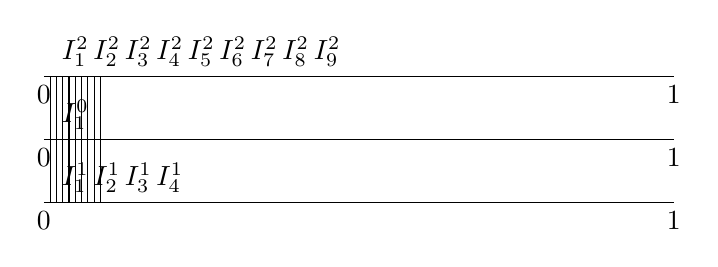
\begin{tikzpicture}[scale=0.8]
    % Draw the horizontal lines
    \draw (0,0) -- (10,0);
    \draw (0,1) -- (10,1);
    \draw (0,2) -- (10,2);

    % Label the endpoints
    \node at (0,0) [below] {$0$};
    \node at (10,0) [below] {$1$};
    \node at (0,1) [below] {$0$};
    \node at (10,1) [below] {$1$};
    \node at (0,2) [below] {$0$};
    \node at (10,2) [below] {$1$};

    % Draw the vertical lines for the partitions
    \foreach \x in {1,2,...,9} {
        \draw (\x/10,0) -- (\x/10,1);
        \draw (\x/10,1) -- (\x/10,2);
    }

    % Label the intervals
    \node at (1/2, 1) [above] {$I^0_1$};
    \node at (1/2, 0) [above] {$I^1_1$};
    \node at (2/2, 0) [above] {$I^1_2$};
    \node at (3/2, 0) [above] {$I^1_3$};
    \node at (4/2, 0) [above] {$I^1_4$};
    \node at (1/2, 2) [above] {$I^2_1$};
    \node at (2/2, 2) [above] {$I^2_2$};
    \node at (3/2, 2) [above] {$I^2_3$};
    \node at (4/2, 2) [above] {$I^2_4$};
    \node at (5/2, 2) [above] {$I^2_5$};
    \node at (6/2, 2) [above] {$I^2_6$};
    \node at (7/2, 2) [above] {$I^2_7$};
    \node at (8/2, 2) [above] {$I^2_8$};
    \node at (9/2, 2) [above] {$I^2_9$};
\end{tikzpicture}

\end{document}